\documentclass[a4paper,10pt,twoside]{report}

% Packages for enhancing LaTeX capabilities
\usepackage[a4paper, inner=4cm, outer=3cm, top=2.5cm, bottom=2.5cm]{geometry}
\usepackage{fontspec}
\usepackage{setspace}
\usepackage{fancyhdr}
\usepackage{graphicx}
\usepackage[backend=biber,style=apa]{biblatex}
\usepackage{csquotes}
\usepackage[ngerman]{babel}
\usepackage{float}
\usepackage{amsmath}



\setmainfont{Arial}
\setstretch{1.2}
\pagenumbering{roman}
\setcounter{page}{1}
\addbibresource{../../Ressourcen/Bibliographie/ba_literatur.bib}


\begin{document}

% Titlepage
\begin{titlepage}
  \hspace*{\fill}
  
\includegraphics[width=0.4\textwidth,keepaspectratio]{../../Ressourcen/Bilder/FHE-AI_Logo.png}

  \centering
  \vspace*{1cm}

  \vspace{0.5cm}

  {\Huge\textbf{Bachelorarbeit in der Angewandten Informatik}}
  \\
  Registriernummer: AI-2024-BA-030

  \vspace{1.5cm}

  {\large\textbf{Konzeption und Entwicklung einer datenbankseitigen Abbildung von frei definierbaren Bilanzräumen
      im Zusammenhang mit dem Energiemanagementsystem EMS-EDM PROPHET® nach ISO 50001.}}

  \vspace{1.5cm}

  {\Large\textbf{Fabian Heinlein}}
  \\ in Kooperation mit dem Fraunhofer Institut Angewandte Systemtechnik (IOSB-AST)

  \vspace{1cm}

  \Large Abgabedatum: 28.02.2024

  \vspace{1cm}

  Prof. Dr. Marcel Spehr \\
  Sven Möller

  \vfill

\end{titlepage}



\chapter*{Kurzfassung}
\addcontentsline{toc}{chapter}{Kurzfassung}
\chapter*{Abstract}
\addcontentsline{toc}{chapter}{Abstract}
\chapter*{Vorwort}
\addcontentsline{toc}{chapter}{Vorwort}
\tableofcontents

%%%%%%%%%%%%%%%%%%%%%%%%%% Einleitung %%%%%%%%%%%%%%%%%%%%%%%%%%
\chapter{Einleitung}
\pagenumbering{arabic}
\setcounter{page}{1}

\section{Hintergrund und Motivation}
Angesichts wachsender Umweltbelastungen und der Notwendigkeit nachhaltiger Praktiken spielt das Energiemanagement eine immer bedeutendere Rolle.
Diese Arbeit untersucht die Entwicklung einer datenbankseitigen Lösung zur Abbildung frei definierbarer Bilanzräume im Energiemanagementsystem
EMS-EDM PROPHET® nach DIN EN ISO 50001:2018-12.
Sie wird durch das Potenzial, bei der Verbesserung der energiebezogenen Leistung und Energieeffizienz von Organisationen im tertiären Wirtschaftssektor 
durch die Erfüllung ausgewählter Kriterien der DIN EN ISO 50001:2018-12 zu unterstützen, motiviert. 
Bilanzräume stellen das zentrale Konzept der Arbeit dar und werden im Rahmen dieser als Einheiten betrachtet, die zur digitalen Abbildung 
von Organisationsstrukturen im Energiemanagement und als administrative Grenze zur Bilanzierungsrechnung dienen.
Die Adressierung der Arbeit auf die freie definierbare Gestaltung der Bilanzräume soll eine Möglichkeit bieten, der Diversität von Organisationen innerhalb des 
tertiären Wirtschaftssektors gerecht zu werden
und einen Einsatz der Forschungsergebnisse in solchen Organisationen mit dem EDM-EMS-Prophet® ermöglichen.
Die Untersuchung soll zur Weiterentwicklung nachhaltiger Energiemanagementpraktiken beitragen und Einblicke in die Integration
technischer Lösungen in bestehende Systeme bieten.

Ein wesentlicher Fokus dieser Arbeit liegt auf der DIN EN ISO 50001:2018-12, einer Norm der Internationalen Organisation für Normung (ISO),
die Anforderungen an Energiemanagementsysteme festlegt. Diese Norm ist universell einsetzbar, unabhängig von Größe, Art oder Standort der Organisation (\cite[S. 10]{DIN50001.2018}),
und dient der fortlaufenden Verbesserung der energiebezogenen Leistung. (\cite[S. 7]{DIN50001.2018}).
Um die Anforderungen der DIN EN ISO 50001:2018-12 zu erfüllen, müssen Organisationen den kontinuierlichen Fortschritt ihrer energiebezogenen Leistung nachweisen, wobei
die Norm keine spezifischen Zielniveaus vorgibt. (\cite[S. 10]{DIN50001.2018}).

Die Umsetzung der DIN EN ISO 50001:2018-12 in Organisationen bringt sowohl operationale als auch organisatorische Herausforderungen mit sich [S. 11](\cite{Marimon.2017}).
Dennoch lag im Jahr 2023 in 24.924 Organisationen weltweit ein Zertifikat nach DIN EN ISO 50001:2018-12 vor (\cite{InternationalOrganizationforStandardization.2023}).
Dies ist bemerkenswert, da die Erfüllung der Normanforderungen voraussichtlich etwa 60 \% des globalen Energieverbrauchs beeinflussen
kann (\cite{InternationalOrganizationforStandardization.2011}, zitiert nach \cite[S. 1]{Marimon.2017}). Darüber hinaus entstehen für Organisationen durch
die Einführung der Norm signifikante Vorteile.

Zum einen können nach Aussagen der DIN EN ISO 50001:2018-12 (2018, S. 9) ökonomische Vorteile wie Energieeinsparungen erzielt werden, wodurch Organisationen einen Wettbewerbsvorteil
aufgrund sinkender Energiekosten erlangen können. Zum anderen ergeben sich operationale Vorteile wie eine gesteigerte Produktivität, verbesserte Qualität
und ein strukturierter Ansatz zur Prozessoptimierung (\cite{Marimon.2017}). Des Weiteren kann die Umsetzung der DIN EN ISO 50001:2018-12 dazu beitragen, die allgemeinen
Klimaschutzziele zu erreichen (\cite{DIN50001.2018}). Dies unterstreicht die gesellschaftliche Bedeutung der Norm, insbesondere angesichts der Herausforderungen
des Klimawandels.

Die Umsetzung der DIN EN ISO 50001:2018-12 basiert auf dem PDCA-Zyklus (Plan, Do, Check, Act), der Organisationen einen strukturierten Rahmen für die fortlaufende
Verbesserung der energiebezogenen Leistung bieten soll (\cite[S. 7f.]{DIN50001.2018}).
Während die Norm in erster Linie Anforderungen auf Managementebene formuliert, verweist sie auch auf technische Normen wie die E DIN ISO 50006:2024-07, die unter anderem
spezifische Anforderungen an Energieleistungskennzahlen und energetische Ausgangsbasen definiert (\cite{DIN50006.2024,DIN50001.2018}).


\section{Problemstellung}
\subsection{Problembeschreibung}
\textbf{Forschungsfrage:} "Welche strukturellen Erweiterungen und Anpassungen müssen auf Datenbankebene in EMS-EDM PROPHET® konzipiert und implementiert 
werden, um eine frei definierbare Abbildung von Bilanzräumen zu ermöglichen, die Organisationen bei der Erfüllung der ISO 50001 unterstützt?"

Die breite Anwendbarkeit der in der DIN EN ISO 50001:2018-12 gestellten Anforderungen auf Organisationen führt zu Anforderungen an die Abbildbarkeit von 
frei definierbaren energiebezogenen Organisationsstrukturen im Energiemanagementsystem.

Ein Teilaspekt zur Umsetzung der DIN EN ISO 50001:2018-12 im Rahmen der Energiebilanzierung ist die Abbildung von energiebezogenen Bereichen in 
Organisationen im Energiemanagementsystem und soll im Rahmen dieser Arbeit betrachtet werden.

Die aktuelle Datenbankstruktur von EMS-EDM Prophet® steht vor dem Problem, frei definierbare Bilanzräume abzubilden.
Um dieses Problem zu lösen, sind strukturelle Änderungen und Erweiterungen der Datenbank notwendig.
Somit besteht das zentrale Problem dieser Arbeit darin, ein System zur Abbildung frei definierbarer Bilanzräume auf Datenbankebene unter Berücksichtigung 
der von der DIN EN ISO 50001:2018-12 gestellten Anforderungen an Bilanzräume und damit verbundene Themenkomplexe in EMS-EDM Prophet® zu konzipieren und 
zu implementieren.

Die Problemlösung umfasst alle Aspekte, die auf Grundlage der Vorgaben der Norm sowie praktischer Gegebenheiten konzipiert und auf Datenbankebene 
umgesetzt werden müssen, um EMS-EDM PROPHET® so zu erweitern, dass das System in der Lage ist, Organisationen bei der Erfüllung der ISO 50001 zu 
unterstützen. Dies gilt insbesondere für Anforderungen, die durch die Abbildung von Bilanzräumen adressiert werden können.

Aufgrund der Anwendbarkeit der DIN EN ISO 50001:2018-12 auf alle Organisationen ist die freie Definierbarkeit der Bilanzräume ein Qualitätskriterium des zu 
entwerfenden Systems und spielt bei der Beantwortung der Forschungsfrage eine zentrale Rolle.
Die breite Anwendbarkeit der Norm impliziert außerdem die Notwendigkeit, praktische Herausforderungen beim Einsatz der Lösung zu berücksichtigen und 
Anwendungsgebiete des entworfenen Konzepts zu betrachten, um der praktischen Relevanz dieser Arbeit gerecht zu werden.

\subsection{Praktische Relevanz des Problemraums} 
Das beschriebene Problem weist eine praktische Relevanz auf, da es die Herausforderungen der DIN EN ISO 50001:2018-12
im Energiemanagement von Organisationen adressiert.
Die bestehenden Anforderungen der DIN EN ISO 50001:2018-12 und der aktuelle Zustand von EMS-EDM Prophet® stellen praxisnahe Qualitätskriterien an die Abbildung von Bilanzräumen.
Eine Herausforderungen besteht darin, ein Datenbankmodell zu entwickeln, das diese Anforderungen erfüllt und gleichzeitig praxisnah und umsetzbar ist.
Die Berücksichtigung von aus der Praxis abgeleiteten Anforderungen ist dabei unerlässlich.
Dies verdeutlicht die Notwendigkeit einer Methodik, die sowohl theoretische als auch praktische Aspekte integriert.
Die Integration der Lösung in EMS-EDM Prophet® stellt sicher, dass sie in bestehenden Organisationen nutzbar ist und deren Energiemanagement unterstützt.

\subsection{Wissenschaftliche Relevanz des Problemraums} 
Die Problemstellung weist eine wissenschaftliche Relevanz auf, da im Zuge der Erarbeitung einer Lösung Methoden des Datenmanagements im Kontext der 
Modellierung von Energiebilanzräumen angewandt werden.
Dabei werden die in EMS-EDM Prophet® bestehenden Methoden um neue Ansätze zur Modellierung von Bilanzräumen erweitert.
Diese Erweiterungen tragen zur wissenschaftlichen Diskussion über Datenmanagementstrategien im Energiemanagement bei und bieten neue Perspektiven für die 
Integration von Bilanzräumen in datenbankbasierte Systeme.
Darüber hinaus fördert die Arbeit den interdisziplinären Austausch zwischen den Bereichen Energiemanagement und Datenbankmodellierung, indem sie 
theoretische Konzepte mit praktischen Anwendungen verknüpft.
Die entwickelten methodischen Ansätze und Modelle können als Grundlage für zukünftige wissenschaftliche Untersuchungen dienen und die Weiterentwicklung 
von Energiemanagementsystemen unterstützen.


\section{Ziel der Arbeit}

Das Ziel dieser Arbeit ist die Konzeption, Implementation und Evaluation eines Prototyps, der durch strukturelle Anpassungen und 
Erweiterungen des EMS-EDM Prophet® die Abbildung frei definierbarer Bilanzräume ermöglicht. Der Prototyp soll einen Mehrwert zur 
Erfüllung der Anforderungen der DIN EN ISO 50001:2018-12 bieten und in Organisationen des tertiären Wirtschaftssektors, die EMS-EDM Prophet® nutzen, 
anwendbar sein. Die Erarbeitung des Prototyps soll auf den theoretischen Grundlagen des Daten- und Energiemanagements basieren und bewährte Ansätze 
aus den Bereichen verwenden. Außerdem soll der Prototyp praktische Herausforderungen in den potentiellen Anwendungsgebieten berücksichtigen und 
allgemeine Anforderungen an Organisationen zu dessen Umsetzung formulieren.


Zur Evaluation des Prototyps soll die Bilanzraumstruktur der Organisation: Fraunhofer IOSB-AST in Ilmenau im entworfenen Prototyp abgebildet werden.
Der angewendete Prototyp soll im Bezug auf die unterstützung bei der Erfüllung der DIN EN ISO 50001:2018-12 Anforderungen auf qualitative und quantitative 
Qualitätskriterien evaluiert werden.
Außerdem soll die freie Definierbarkeit und die praktische Anwendbarkeit des Prototyps evaluiert werden.



\section{Aufbau der Arbeit}
Diese Arbeit ist so konzipiert, dass Sie die theoretischen Grundlagen des Problemraums erfasst und Nutzen sowie Herausforderungen im Anwendungsgebiet: 
EMS nach DIN EN ISO 50001:2018-12 erarbeitet. 
Basierend auf den theoretischen Grundlagen im Anwendungsbereich und den bestehenden Methoden und Ansätzen des Datenmanagements 
in EMS-EDM Prophet® wird eine Lösung der Forschungsfrage auf Datenbankebene des Energiemanagementsystems konzipiert, 
implementiert und evaluiert.
Der Aufbau der Arbeit umfasst drei Hauptabschnitte: die theoretischen Grundlagen und der Stand der Wissenschaft, die Konzeption und Implementation, und die 
Evaluation.

\begin{enumerate}
    \item \textbf{Theoretische Grundlagen und Stand der Wissenschaft}
    
    Die praxisnahe Problemstellung erfordert eine anwendungsorientierte Forschung unter Berücksichtigung der Interdisziplinarität. 
    Im theoretischen Teil der Arbeit werden zwei Themenbereiche betrachtet: Grundlagen der Energiebilanzierung unter Nutzung von Bilanzräumen und  
    Energiemanagementsysteme nach DIN EN ISO 50001:2018-12. In beiden Tehemenbereichen findet die erarbeitung der Grundlagen unter beachtung des Anwendungsgebiets: 
    Organisation im tertiären Wirtschaftssektor statt. 
    
    Für die Erarbeitung der theoretischen Grundlagen des Energiemanagements werden im ersten Hauptabschnitt der Arbeit die DIN EN ISO 50001:2018-12, 
    damit verbundene Normen und Basiswissen aus für den Problemraum relevanter Fachliteratur analysiert.
    Außerdem werden wissenschaftliche Arbeiten aus verwandten Problemräumen analysiert und in den Kontext dieser Arbeit gesetzt.
    Auf dieser Basis werden theoretische Konzepte und Anforderungen aus dem Problemraum abgeleitet, die für die Lösung der Forschungsfrage relevant sind.
    
    Der erste Hauptabschnitt der Arbeit hat somit eine zentrale Bedeutung zum erreichen der Interdisziplinarität der Forschung.
    Die umfangreiche erarbeitung von Konzepten des Energiemanagements, Anforderungen von Anforderungen der ISO 50001 und den Einsatzmöglichkeiten 
    von Bilanzräumen zur praxisnahen erfüllung dieser Anforderungen auf basis der Konzepte stellen eine detaillierte Analyse des Anwendungsbereichs dieser 
    Forschung dar.
    Diese Detaillierte Analyse, ohne technische Perspektive der Datenbankmodellierung, ist notwendig um der Interdisziplinarität des Problemraums aus Sicht des 
    Energiemanagements und der Energiebilanzierung gerecht zu werden. 
    Die erarbeiteten Grundlagen des Anwendungsbereichs: Energiemanagent wird im nächsten Hauptabschnitt, der Konzeption und Implementation, 
    aufgegriffen und aus einer technischen Sicht des Datenbankmanagements betrachtet.

    \item \textbf{Konzeption und Implementation des Prototyps}

    Basierend auf den Forschungsergebnissen des theoretischen Teils der Arbeit wird im zweiten Kapitel der Arbeit eine Lösung für den Problemraum
    konzipiert und implementiert.
    Um der Interdisziplinarität aus Sicht der Datenbankmodellierung gerecht zu werden, wird der IST-Zustand des EMS-EDM Prophet® analysiert und es werden 
    bereits bestehende Ansätze der Datenbankmodellierung die den Problemraum addressieren aufgezeigt.
    Unter berücksichtigung der aufgezeigten Ansätze wird der Prototyp zur Problemlösung konzipiert und EMS-EDM Prophet® im implementiert.
    Im Zuge dessen ist die konzeption und integration von Ansätzen des Datenbankmanagements, die noch nicht im EMS-EDM Prophet® bestehen 
    notwendig.
    Das Konzept addressiert die im ersten Hauptabschnitt erarbeiteten Erkenntnisse des Anwendungsbereichs: Energiemanagement und Energiebilanzierung 
    und stellt eine Datenbankseitige abbildung der Grundsätze unter den erarbeiteten Anforderungen der ISO 50001 im kontext von Organisationen des 
    tertiären Wirtschaftssektors zur verfügung.
    
    \item \textbf{Evalutation des Prototyps}
    
    Im dritten Hauptabschnitt der Arbeit wird der entworfene Prototyp evaluiert.
    Im Zuge dessen wird die Bilanzraumstruktur des Fraunhofer IOSB-AST in Ilmenau erarbeitet und im entworfenen Prototyp abgebildet.
    Anhand dieses praktischen Beispiels wird getestet wie korrekt die im ersten Hauptabschnitt erläuterten Methoden des Energiemanagements und der Energiebilanzierung 
    umgesetzt wurden, und wie der Prototyp in der Praxis bei der Erfüllung von ISO 50001 Anforderungen Organisationen unterstützen kann. 
    Dieser Abschnitt der Evaluation findet unter Nutzung quantitativer Qualitätskriterien statt.

    Des weiteren wird grundsätzlich betrachtet, wie im Rahmen der Interdisziplinarität die im ersten Hauptabschnitt erarbeiteten Erkenntnisse aus Sicht 
    des Energiemanagements technisch durch den konzipierten und implementierten Prototyp abgebildet wurde.
    Dabei wird auch analysiert ob und wie die im ersten Hauptabschnitt erörterten Anforderungen der ISO 50001 auf Datenbankebene umgesetzt wurden sind.
    Dieser Abschnitt der Evaluation findet unter Nutzung qualitativer Qualitätskriterien statt.

\end{enumerate}


%%%%%%%%%%%%%%%%%%%%%%%%%% Theoretische Grundlagen %%%%%%%%%%%%%%%%%%%%%%%%%%

\chapter{Theoretische Grundlagen}
\section{Modellierung von Bilanzräumen}

\subsection{Grundlagen von Bilanzräumen}

\subsubsection{Definition von Bilanzräumen}
Energiebilanzräume stellen ein zentrales Konzept im Energiemanagement dar und bilden die Grundlage für die Berechnung von Energieleistungskennzahlen, da sie deren Vergleichbarkeit sicherstellen [\cite[Kapitel 5.4.2]{Engelmann.2015}]. 
Sie umfassen laut Engelmann (2015) sowohl Energiequellen als auch Energiesenken und müssen anhand einheitlicher Kriterien definiert werden müssen. Des Weiteren besteht die Möglichkeit, 
Bilanzräume in mehrere Teilbilanzräume zu unterteilen [\cite[Kapitel 5.4.2]{Engelmann.2015}].

% TODO: Praxisbeispiel Bilanzraumzerlegung mit ableitung von Methodischen Ansätzen + breitere Quellen


\subsubsection{Bilanzierung}
Bilanzräume haben unter anderem eine Relevanz für die Bilanzierung in Organisationen. Eine Bilanzierung bezeichnet in diesem Kontext die Berechnung der in einen Bilanzraum ein- und austretenden 
Energieflüsse [\cite[S. 65]{Rönsch.2015}]. Nach der Definition von Engelmann (2015, Kapitel 5.4.2) muss dabei die Summe der Energiequellen und -senken eine Null-Bilanz ergeben. Im Rahmen des Energiemanagements steht 
die Energiebilanz im Fokus. Die Energiebilanzierung ist laut Rönsch (2015, S. 66) eine Form der Bilanzierung die auf dem Prinzip der Energieerhaltung beruht, welcher besagt, dass die Energie in einem abgeschlossenen System, über die Zeit 
konstant ist. Abgeschlossen meint in diesem Kontext wärmeundurchlässig. Für abgeschlossene Systeme ohne Speicherkapazitäten bedeutet das dass die Summe der Energiequellen gleich der Summe der Energiesenken ist, 
sollte das System über Energiespeicherkapazitäten verfügen so ist die Menge der gespeicherten Energie gleich der Differenz aus der Summe der Energiequellen und -senken [\cite{Rönsch.2015}]. 

Die Energiebilanz nach Rönsch (2015) lässt sich mathematisch mit der folgenden Gleichung darstellen:

\[
E_{\text{gespeichert}} = \sum E_{\text{quelle}} - \sum E_{\text{senke}}
\]

\textbf{Erläuterung der Gleichung:}
\begin{itemize}
    \item \(E_{\text{gespeichert}}\): Energie, die im System gespeichert wird.
    \item \(\sum E_{\text{quelle}}\): Summierte zugeführten Energie, der Energiequellen.
    \item \(\sum E_{\text{senke}}\): Summe aller Energiesenken, also der verbrauchten Energie.
\end{itemize}

Für abgeschlossene Systeme ohne Energiespeicher  gilt:
\[
E_{\text{gespeichert}} = 0
\]
In diesem Fall ist die zugeführte Energie gleich der verbrauchten Energie:
\[
\sum E_{\text{quelle}} = \sum E_{\text{senke}}
\]

%TODO: Praxisbeispiel mit Anwendung der Gleichung


\subsubsection{Energiequellen und -senken}


Die definition von Bilanzräumen mit den zu bilanzierenden Energiequellen und -senken kann grundlegend für den Aufbau eines Energieflussmodells verwendet werden. 
Ein Energieflussmodell berechnet die Massen- und Energiebilanzen sowie die thermodynamischen Gleichgewichtsbedingungen der Komponenten [\cite{FrancescaPalazzi.2007}] und stellt somit eine zentrale Komponente 
zur Energeiebilanzierung in Organisationen.


\subsubsection{Beziehungen zwischen Bilanzräumen}


\subsubsection{Praktische Herausforderung im Zusammenhang mit Bilanzräumen}
Die Definition von Bilanzräumen, wie sie von Engelmann (2015, Kapitel 5.4.2) beschrieben wird, bildet eine wesentliche Grundlage für die Analyse und Optimierung der energiebezogenen Leistung von Organisationen. 
Dabei müssen die Bilanzraumkriterien den spezifischen Gegebenheiten der Organisation angepasst werden. Dies wird deutlich, wenn man den Energieverbrauch in verschiedenen Sektoren betrachtet.

\begin{figure}[H]
    \centering
    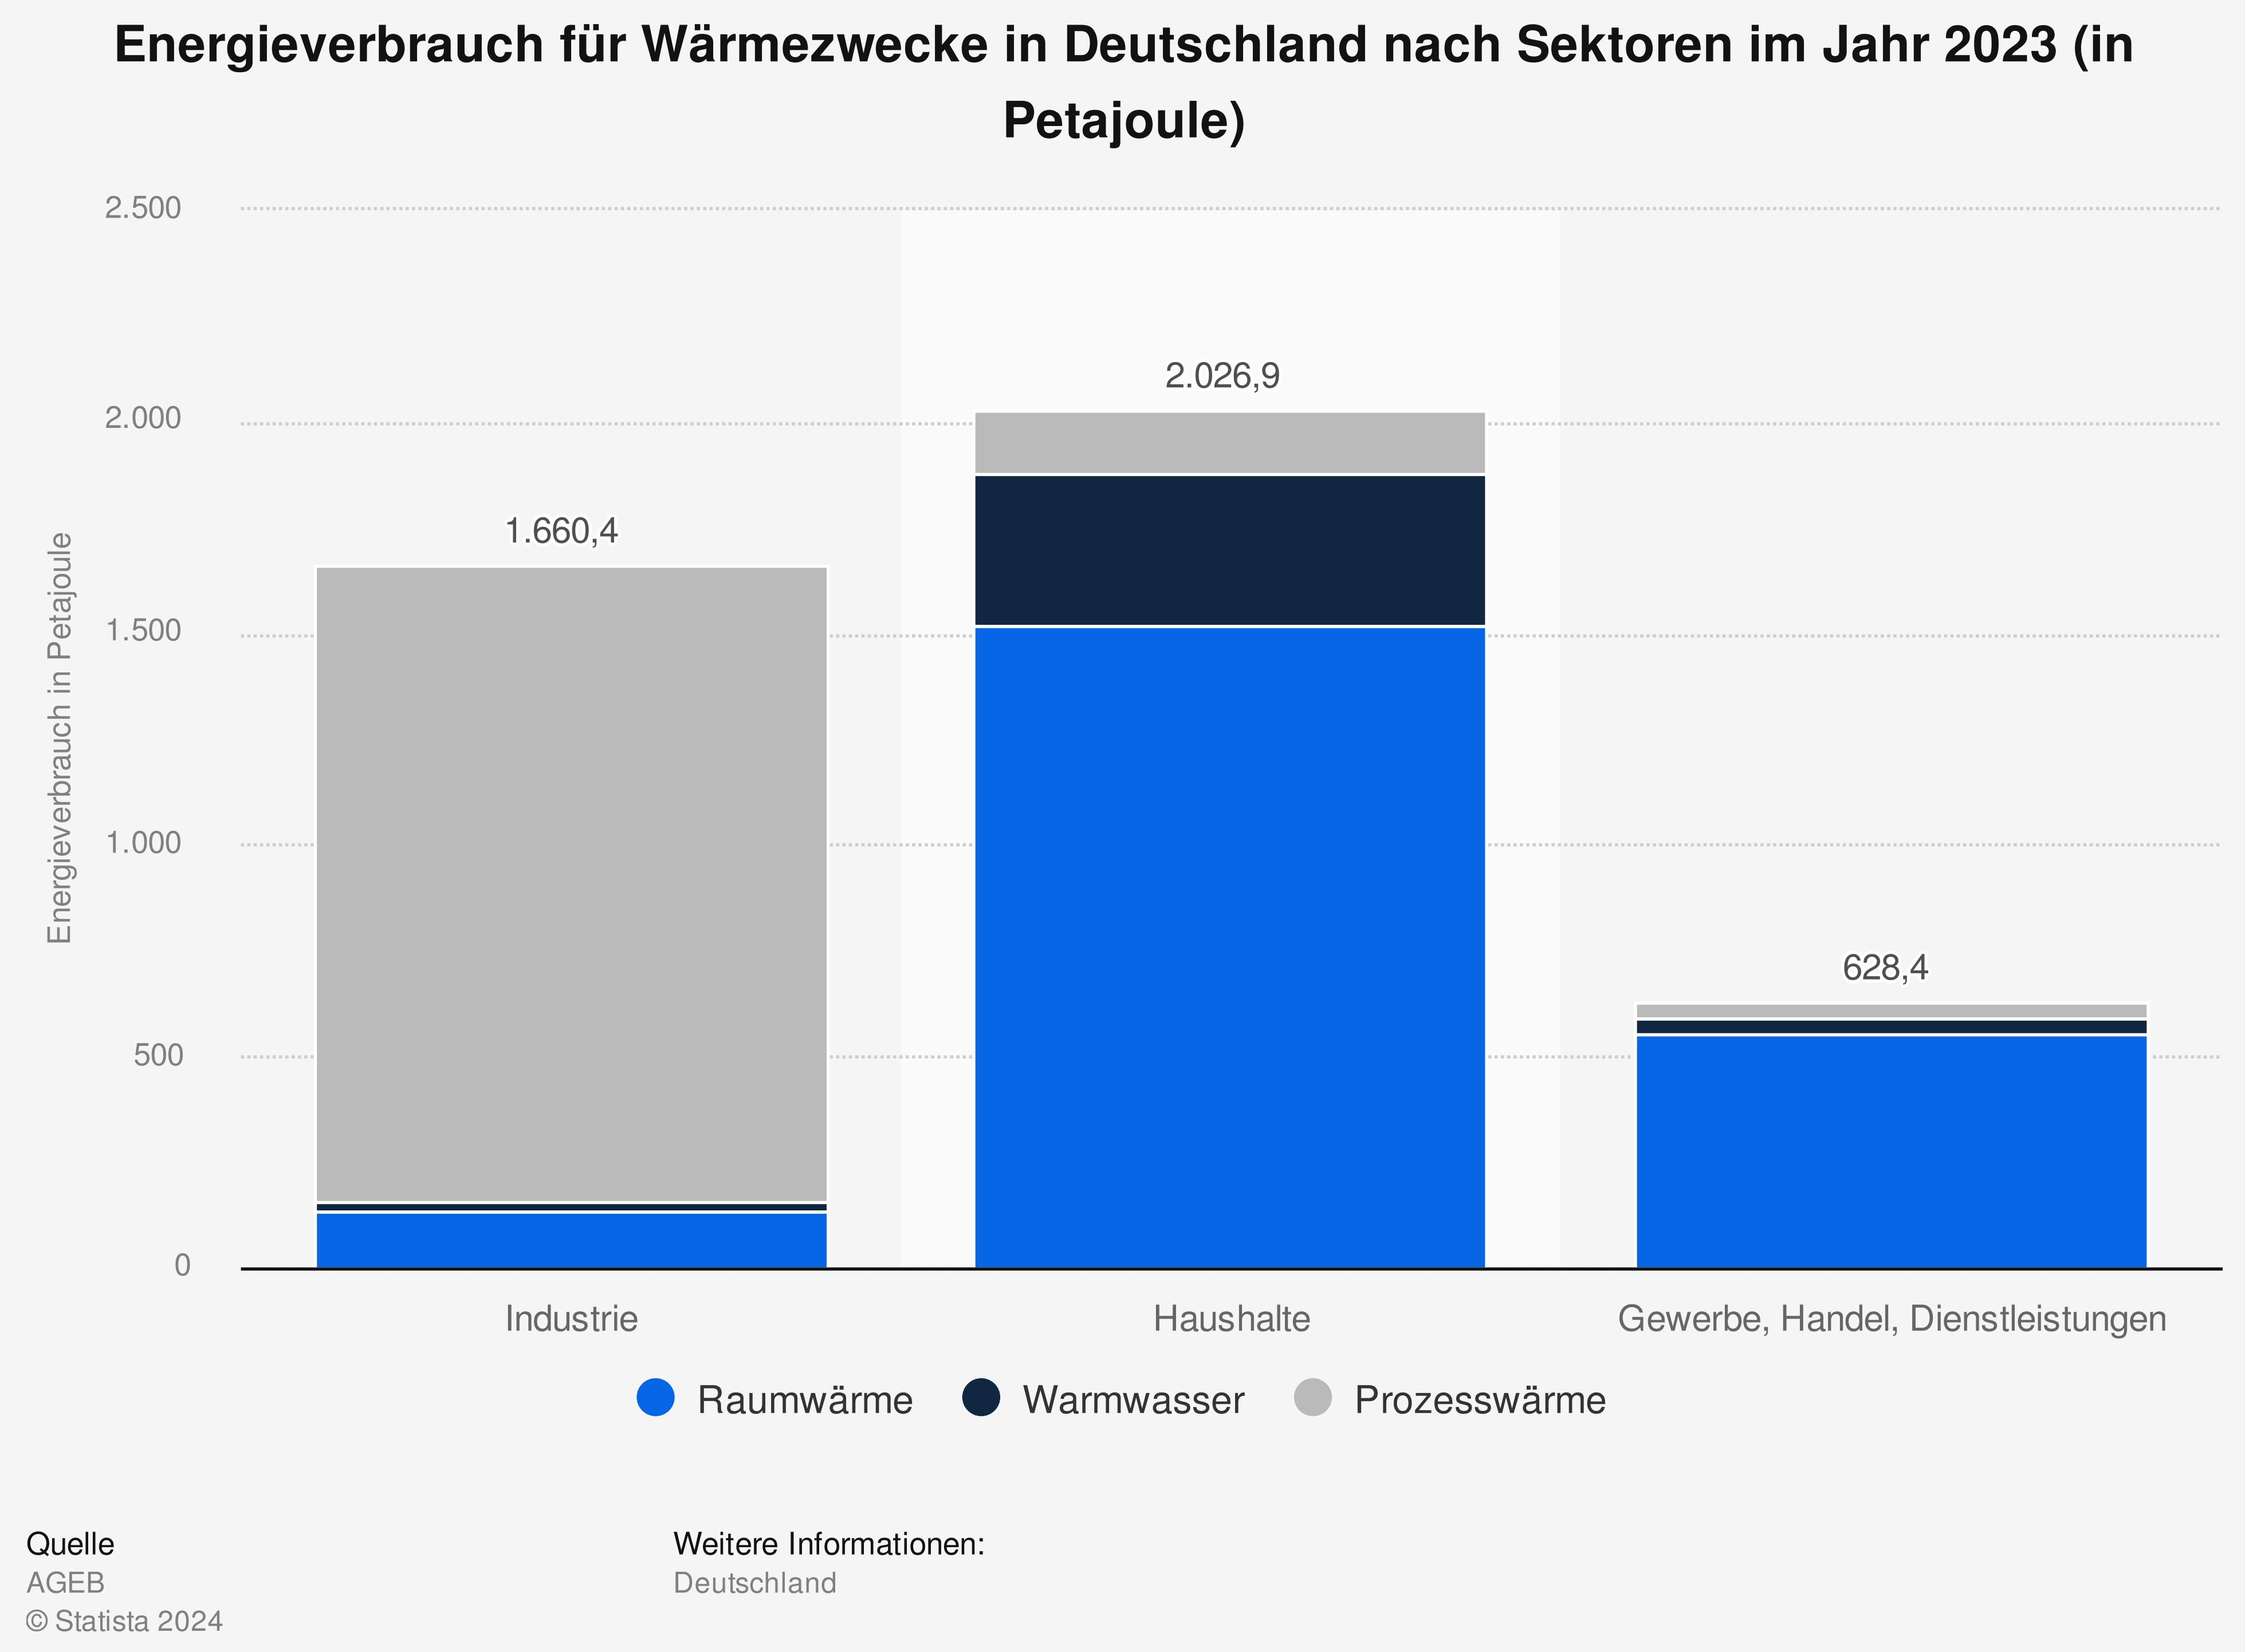
\includegraphics[width=1\textwidth]{../../Ressourcen/Bilder/Energieverbrauch_für_Wärmezweck_DE.jpg}
    \caption{Energieverbrauch für den Wärmezweck in Deutschland [\cite{AGEB.2024}]}
    \label{fig:Energieverbrauch_Wärme_DE}
\end{figure}

Abbildung \ref{fig:Energieverbrauch_Wärme_DE} zeigt den Energieverbrauch für Wärmezwecke in Deutschland im Jahr 2023, aufgeschlüsselt nach Sektoren. Hieraus lassen sich grundlegende Erkenntnisse für die 
praktische Definition von Bilanzräumen ableiten. Der industrielle Sektor weist einen hohen Anteil an prozessbezogener Wärme auf, was darauf hinweist, dass hier spezifische Bilanzräume für die Erfassung und 
Optimierung von Prozesswärme sinnvoll sind. Im Gegensatz dazu spielt im Dienstleistungssektor die Raumwärme eine dominierende Rolle denn in Organisationen, die immaterielle Dienstleistungen 
erbringen, spielt die Gebäudeenergie eine entscheidende Rolle bei der Verbesserung der energiebezogenen Leistung, während Prozesse oder Technologien eine untergeordnete Bedeutung haben [\cite{AlbertoFichera.2020}]. 
Dies erfordert andere Schwerpunkte bei der Definition von Bilanzraumkriterien.

Dieser Unterschied zeigt, dass ein einheitlicher Ansatz zur Definition von Bilanzraumkriterien sektorenübergreifend nicht zielführend ist. Stattdessen sollten die Bilanzraumkriterien auf den jeweiligen Energieeinsatz 
abgestimmt werden, um Optimierungspotenziale gezielt identifizieren zu können. Für Organisationen, die Dienstleistungen anbieten, bedeutet dies beispielsweise, dass die Gebäudeenergie als zentrale Energiesenke 
in den Fokus rückt, während bei Industriebetrieben die Energieflüsse innerhalb der Produktionsprozesse detaillierter bilanziert werden sollten.

%Ausblick: welche Relevanz haben Interdepenzen von Energiequellen und - Senken 

\subsection{Bilanzräume im Energiemanagementsystem}
\subsection{Ansätze zur Datenbankseitigen Modellierung}


\section{Bewertung der energiebezogenen Leistung eines Bilanzraums}

\subsection{Grundlagen der Energiebezogenen Leistung}

\subsection{Energieleistungskennzahlen}

\subsection{Energetische Ausgangsbasen}

\subsection{Ansätze zur Datenbankseitigen Auswertung}

\section{Technische Anforderungen im Organisationskontext}

\subsection{Grundlagen der technischen Anforderungen}

\subsection{Energiedatensammlung nach ISO 50001}

\subsection{Stammdatenverwaltung nach ISO 50001}

\subsection{Umsetzung im Organisationskontext}


%%%%%%%%%%%%%%%%%%%%%%%%%% Konzept %%%%%%%%%%%%%%%%%%%%%%%%%%

\chapter{Konzeption und implementation in EMS-EDM Prophet®}
\section{Einleitung}

\section{Ausgangszustand: EMS-EDM Prophet®}

\section{Anforderungen}
\subsection{Modellierung von Bilanzräumen}

\subsection{Abbildung von Metriken zur Bewertung von Bilanzräumen}

\subsection{Technische Anforderungen und Datenkommunikation}


\section{Umsetzungskonzept für EMS-EDM Prophet®}

\subsection{Systemarchitektur}
\subsection{Datenmodell und Datenbankdesign}
\subsection{Technische Umsetzung und Datenkommunikation}
\subsection{EnPI Abbildung}
\subsection{Test- und Validierungskonzept}
\subsection{Sicherheitskonzept}
\subsection{Bedingungen und Anforderungen an die Laufzeitumgebung}

\section{Technische Realisierung}
In diesem Kapitel sollen alle technischen Aspekte der Umsetzung beschrieben werden.
\section{Umsetzungsablauf}
In diesem Kapitel soll der Ablauf der Umsetzung beschrieben und begründet werden.
\section{Ergebnis}
In diesem Kapitel soll das Ergebnis der Umsetzung beschrieben werden.
\subsection{Anforderungsumsetzung}
In diesem Kapitel soll beschrieben werden wie die Anforderungen umgesetzt wurden und welche Anforderungen umgesetzt wurden.
\subsection{Vergleich zum bestehenden System}
In diesem Kapitel soll der Vergleich zum bestehenden System gezogen werden und erläutert werden was sich verändert hat.


%%%%%%%%%%%%%%%%%%%%%%%%%% Implementation und Evaluation %%%%%%%%%%%%%%%%%%%%%%%%%%

\chapter{Evaluation}

\section{Einleitung}
\subsection{Ziel der Evaluation}
\subsection{Methodik}

\section{Metriken und Kennzahlen}
\subsection{Definition der Erfolgsmessung}
\subsection{Quantitative Metriken}
\subsection{Qualitative Metriken}

\section{Experimenteller Aufbau}
\subsection{Beschreibung des Experimentes}
\subsection{Testumgebung und -bedingungen}
\subsection{Datensätze und Szenarien}

\section{Durchführung und Ergebnisse}
\subsection{Durchführung}
\subsection{Quantitative Ergebnisse}
\subsection{Qualitative Ergebnisse}

\section{Vergleich mit alternativen Ansätzen}

\section{Diskussion der Ergebnisse}

\section{Zusammenfassung der Evaluation}

\chapter{Fazit}
\section{Zusammenfassung der Ergebnisse}
\section{Ausblick auf zukünftige Arbeiten}

\printbibliography[title={Literaturverzeichnis}]

\appendix
\chapter{Anhang}
\section*{Selbstständigkeitserklärung}

\end{document}
